\documentclass[tikz,border=3pt]{standalone}
\usepackage{xcolor}
\usetikzlibrary{arrows.meta,decorations.pathmorphing,positioning}
\definecolor{signalblue}{HTML}{2563EB}
\definecolor{alertred}{HTML}{DC2626}
\definecolor{stagefill}{HTML}{E2E8F0}
\begin{document}
\pgfmathsetseed{100}
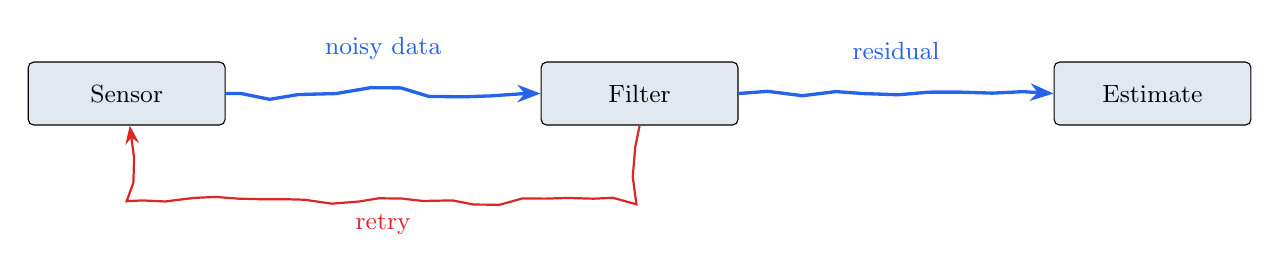
\begin{tikzpicture}[
  >=Stealth,
  stage/.style={draw,rounded corners=2pt,minimum width=2.5cm,minimum height=8mm,fill=stagefill},
  every node/.style={font=\small}
]
  \node[stage] (sensor) {Sensor};
  \node[stage,right=4cm of sensor] (filter) {Filter};
  \node[stage,right=4cm of filter] (estimate) {Estimate};
  \draw[signalblue,very thick,-Stealth,decorate,
    decoration={random steps,segment length=4mm,amplitude=.8mm,pre length=2mm,post length=2mm}]
    (sensor) -- node[above=3mm]{noisy data} (filter);
  \draw[signalblue,very thick,-Stealth,decorate,
    decoration={random steps,segment length=4mm,amplitude=.35mm}]
    (filter) -- node[above=3mm]{residual} (estimate);
  \pgfmathsetseed{41}
  \draw[alertred,thick,-Stealth,decorate,
    decoration={random steps,segment length=3mm,amplitude=.55mm,mirror,raise=.4mm}]
    (filter.south) -- ++(0,-1) -| node[below,pos=.25]{retry} (sensor.south);
\end{tikzpicture}
\end{document}
